\mainsection{3}{Repaso de IS-LM}{9/2/2021}

El modelo IS-LM es un modelo de demanda asi entonces podemos establecer la demanda total de bienes por medio de $Z$:
\begin{equation}
    Z= C+I+G+X-M
\end{equation}

\textbf{Supuestos}
Todas las empresas producen el mismo bien, que puede usarse para consumo, inversión o gasto del estado. Las empresas están dispuestas a ofrecer cualquier cantidad del bien a un precio $P$. Estamos estudiando una economía cerrada.
$$X=M=0$$
\section{Partes de modelo}
\subsection{El consumo}
El consumo depende principalmente del ingreso disponible $Y_{D}$. Por lo tanto
\begin{equation}
    C=C(Y_{D})
\end{equation}
Sabiendo que $C(Y_{D})$ es una función lineal del consumo:

\begin{equation*}
    C = c_{0} + c_{1}(Y-T)
\end{equation*}

Sabiendo esto podemos recordar que $c_{1}$ es la propensión marginal a consumir, que un numero que indica cuanto afecta a unidad adicional de ingreso al consumo; debe ser positivo y menor que uno.

Por otra parte el parámetro $c_{0}$ indica el nivel de susbsextistencia del consumo.

\subsection{Inversión y Gasto Publico}

La inversión la vamos a plantear como una variable exógena:
\begin{equation}
    I=\overline{I}
\end{equation}


El gasto publico, junto con los impuestos $T$ determinan la política fiscal. Al igual que la inversión vamos a suponer que son exógenas:
\begin{align}
    G & =\overline{G}\\
    T &= \overline{T}
\end{align}

\subsection{Análisis de Equilibrio}
Denotamos en el mercado de bienes sabemos que $Y$ es la producción, el equilibrio requiere que la producción sea igual a la demanda. 
\begin{align}
    Y &=Z \\
    &=C+\overline{I}+\overline{G}\\
    &= c_{0} + c_{1}(Y-T)\overline{I}+\overline{G}\\
    \textup{Resolvemos para } Y & \nonumber\\
    Y &=\frac{1}{1-c_{1}}(c_{0}+I+G-c_{1}T)
\end{align}
 
En la ecuación (3.9) podemos partir que el termino $(c_{0}+I+G-c_{1}T)$ es lo que llamamos \textbf{gasto autónomo}; mientras que por otra parte  al termino $=\frac{1}{1-c_{1}}$ lo conocemos como el multiplicador del gasto.

\begin{figure}[H]
    \centering
    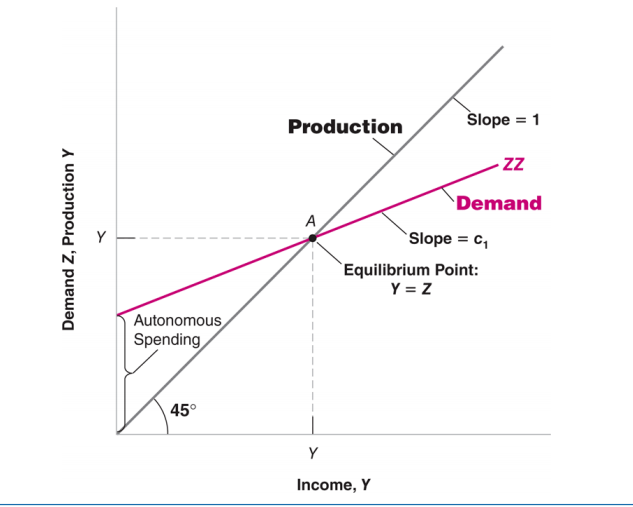
\includegraphics[scale=0.3]{Images/eq_produccion.png}
    \caption{Equilibrio del Mercado de Producción}
    \label{fig:eq_produccion}
\end{figure}

\begin{figure}[H]
    \centering
    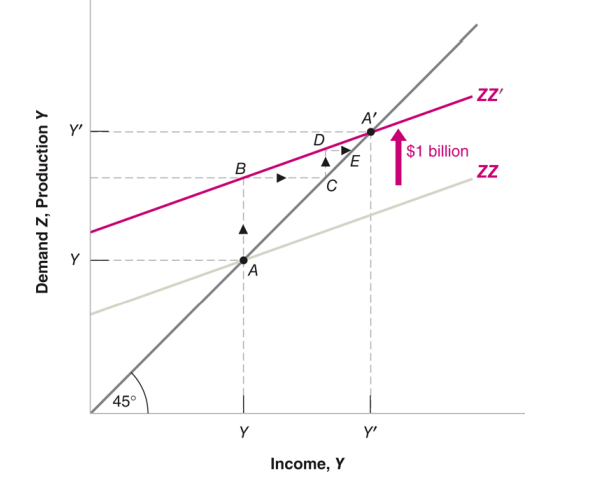
\includegraphics[scale=0.3]{Images/aumento.png}
    \caption{Aumento en Equilibrio del Mercado de Producción}
    \label{fig:auemnto}
\end{figure}

Note que ante un aumento de la demanda inicia un movimiento que finito y repetido en donde el multiplicador del gasto equilibra el merco.

\textbf{Equilibrio en mercado inversion}

Note que el ahorro seria intuitivamente lo que no se consume ni se paga en impuesto. El ahorro (S) es:
\begin{equation}
    S \equiv Y_{D}-C = Y-T-C
\end{equation}

Si lo planteamos en un mercado de bienes: 

\begin{align}
    Y & = C+ G + I\\
    Y-T= C-T+G+I\\
    Y_{D}-C+(T-G) =I\\
    S +(T_G) = I
\end{align}

Esto lo que no dice es que la inversión debe ser igual al ahorro privado (S) y publico. Esta es la relación IS, como Keynes la planteo en la Teoría General.

\subsection{La demanda de dinero}

Suponga que en la economía hay dos activos: dinero y bonos; el \textbf{dinero} puede usarse para realizar transacciones y no rinden intereses. Por lo que hay dos tipos de dinero: \
\begin{itemize}
    \item Efectivo: por su utilidad de cambio
    \item Depósitos a la vista - depósitos bancarios con mentalidad de ahorro
\end{itemize}

Los \textbf{bonos} rinden un tipo de intereses $i$, pero no pueden usarse para realizar transacciones. 

Asi denotamos $M^{d}$ la cantidad de dinero que quieren tener los individuos. Esta demanda depende del nivel de transacciones en la economía. También depende de una función que expresa la preferencia por liquidez. 

\begin{equation}
    M^{d} = \$ Y\underset{(-)}{L(i)}
\end{equation}

Vea como (3.15) se gráfica.

\textbf{Determinación del tipo de interés}

Por simplicidad podemos decir que el equilibrio en el mercado de dinero es cuando la oferta de dinero es igual a la demanda de dinero.

\begin{equation}
    M^{s}=M^{d}
\end{equation}

\textbf{Operaciones de mercado Abierto:} Como el Banco Central interviene en el mercado de dinero, cambiando la oferta monetaria. 

Hay operaciones \textbf{expansivas} y \textbf{contractiva}. 
\begin{itemize}
    \item expansiva compra bonos e inserta dinero en la economía
    \item contractiva vende bono y substrae dinero de la economía
\end{itemize}
 
\textbf{Relación inversa entre precio y tasa de interés}

La relación entre precio y tasa de los bonos es inversa:  Si se analiza si se paga $P$ por un bono $z$ en un año asi el rendimiento es
\begin{equation*}
    i = \frac{1-P}{P}
\end{equation*}

\textbf{La trampa de la liquidez:} existe u limite inferior para la tasa de intereses, por lo que uno piensa que seria una tasa del $0\%$, esto haría que manejar efectivo sea riesgoso y tenga costos añadidos. 

\begin{figure}[H]
    \centering
    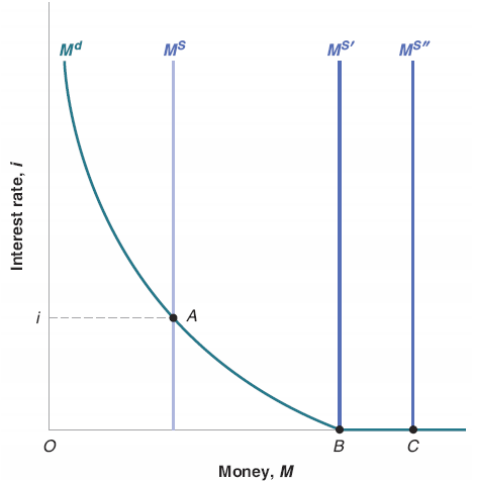
\includegraphics[scale = 0.5]{Images/trampa de liquidez.png}
    \caption{Trampa de liquedez}
    \label{fig:trampa}
\end{figure}
\textbf{Flexibilizando la Inversión:}
La inversión como variable endógena refleja dos factores: 

\begin{itemize}
    \item \textbf{Nivel de ventas:} si las empresas necesitan aumentar su capacidad de producción deben invertir en capital.
    \item \textbf{Tipo de interés:} si las empresas se endeudan, esto afecta su flujo de pagos y su factor de descuento
\end{itemize}

\textbf{Determinación de la producción:} Con el punto anterior la nueva condición de equilibrio se rescata de la forma

\begin{equation}
    Y = C(Y-T)+I(Y,i)+G
\end{equation}

Esta es la relación IS ampliada por inversión, note que ante un aumento en la producción $\implies$ un aumento en el ingreso neto de impuestos que aumenta el consumo. Consecuencia aumenta el nivel de ventas y la inversión.

\subsection{Tasas reales y nominales}

Las tasas de interes pueden expresarse de dos maneras, ya sea de forma nominal en termino de una mondea, en forma real en térmninos de una canaste de bienes. 

\textbf{La diferencia }de ambas esta en, ex-ante, es la inflación esperada. La relación entre estas es respectivamente

\begin{align}
    1 + r_{t} &= (1+i_{t})\frac{P_{t}}{P_{t+1}^{e}} \\
  \textup{La inlfación esperada}  &  \nonumber \\
    \pi_{t+1}^{e} &= \frac{P_{t+1}^{e}-P_{t}}{P_{t}} \\
    \implies &  \nonumber \\
    1 + r_{t} &= \frac{1+i_{t}}{1+\pi_{t+1}^{e}}\\
    r_{t} & \approx i_{t}-\pi_{t+1}^{e} 
\end{align}

La tasa de interés real es relevante pues, los agentes basan sus decisiones en la tasa de interes real. Dicho asi se trae consigo muchas implicaciones ne la política monetaria; asi entonces el Banco Central define la tasa \textbf{nominal} con el objetivo de afectar la tasa \textbf{real}. 

\textbf{Consideremos el riesgo}, ahora podemos partir de un nuevo supuesto de los agentes economicos, y es que deben pagar un prima de riesgo en el mercado de fondos prestables; dicha prima involucra el riesgo de impago y la aversión al riesgo.

Asi si denotamos una función de utilidad podemos definir la función de utilidad esperada, aplicando $x$ prima por riesgo, $p$ probabilidad de impago y tasa de interes libre de riesgo $i$.

\begin{equation}
    U(1+i)= (1-p)U(1+i+x)+ pU(0)
\end{equation}

Podemos ampliar nuestro modelo IS-LM usando el riesgo de la forma que:

\begin{equation}
    Y = C(Y-T)+I(Y, i-\pi^{e}+x)+G
\end{equation}
\myequations{Relación IS Ampliada a Riesgo}

Aplicando la tasa de interes real se ve de la forma
\begin{equation}
    Y = C(Y-T)+I(Y, r+x)+G
\end{equation}